\documentclass[14pt]{article}

\usepackage[utf8]{inputenc}
\usepackage[russian]{babel}
\usepackage{amsmath,amssymb}

\usepackage{geometry}
\geometry{
	a4paper,
	total={170mm,257mm},
	left=20mm,
	top=10mm,
	}

\usepackage{graphicx}
\usepackage{tabularx, ragged2e, booktabs, caption}

\newcommand{\lb}{\left(}
\newcommand{\rb}{\right)}

\newcommand{\mH}{\mathcal{H}}

\newcolumntype{C}[1]{>{\Centering}m{#1}}
\renewcommand\tabularxcolumn[1]{C{#1}}

\begin{document}

Рассмотрим гамильтониан системы $Ar-CO_2$ в молекулярно-фиксированной системе координат:
\begin{gather}
\mH_{mol} = \frac{1}{2 \mu_2} p_R^2 + \lb \frac{1}{2 \mu_2 R^2} + \frac{1}{2 \mu_1 l^2} \rb p_\theta^2 - \frac{1}{\mu_2 R^2} p_\theta J_y + \frac{1}{2 \mu_2 R^2} J_y^2 + \frac{1}{2 \mu_2 R^2} J_x^2 + \frac{1}{2 \sin^2 \theta} \lb \frac{\cos^2 \theta}{\mu_2 R^2} + \frac{1}{\mu_1 l^2} \rb J_z^2 + \notag \\
+ \frac{\ctg \theta}{\mu_2 R^2} J_x J_z + U(R, \theta) \notag
\end{gather}

Выделяя полные квадраты, приходим к следующему выражению:
\begin{gather}
	\mH_{mol} = \frac{p_R^2}{2 \mu_2} + \frac{p_\theta^2}{2 \mu_1 l^2} + \frac{1}{2 \mu_2 R^2} \lb p_\theta - J_y \rb^2 + \frac{1}{2 \mu_2 R^2} \lb J_x + J_z \ctg \theta \rb^2 + \frac{J_z^2}{2 \mu_1 l^2 \sin^2 \theta} + U(R, \theta) \notag
\end{gather}

Произведем следующую линейную замену координат, позволяющую представить отношение гамильтониана к $kT$ в предельно простой форме ($p_R, p_\theta, J_x, J_y, J_z \rightarrow x_1, x_2, x_3, x_4, x_5$, причем $R, \theta$ считаем постоянными при осуществлении замены):
\begin{gather}
	\left\{
	\begin{aligned}
	x_1^2 &= \frac{p_R^2}{2 \mu_2 kT} \\
	x_2^2 &= \frac{p_\theta^2}{2 \mu_1 l^2 kT} \\
	x_3^2 &= \frac{ \lb p_\theta - J_y \rb^2}{2 \mu_2 R^2 k T} \\
	x_4^2 &= \frac{ \lb J_x + J_z \ctg \theta \rb^2}{2 \mu_2 R^2 k T} \\
	x_5^2 &= \frac{J_z^2}{2 \mu_1 l^2 \sin^2 \theta kT}
	\end{aligned}
	\right. \quad \implies \quad 
	\left\{
	\begin{aligned}
	dx_1 &= \frac{dp_R}{\sqrt{ 2 \mu_2 k T}} \\
	dx_2 &= \frac{dp_\theta}{\sqrt{2 \mu_1 l^2 k T}} \\
	dx_3 &= \frac{dp_\theta - dJ_y}{\sqrt{2 \mu_2 R^2 k T}} \\
	dx_4 &= \frac{dJ_x + \ctg \theta dJ_z}{ \sqrt{2 \mu_2 R^2 k T}} \\
	dx_5 &= \frac{dJ_z}{\sqrt{2 \mu_1 l^2 \sin^2 \theta k T}}
	\end{aligned}
	\right. \quad \implies \quad
	\left\{
	\begin{aligned}
		dp_R &= \sqrt{2 \mu_2 k T} dx_1 \\
		dp_\theta &= \sqrt{2 \mu_1 l^2 kT} dx_2 \\
		dJ_y &= \sqrt{2 \mu_1 l^2 kT} dx_2 - \sqrt{2 \mu_2 R^2 kT} dx_3 \\
		dJ_x &= \sqrt{2 \mu_2 R^2 kT} dx_4 - \sqrt{2 \mu_1 l^2 \cos^2 \theta kT} dx_5 \\
		dJ_z &= \sqrt{2 \mu_1 l^2 \sin^2 \theta kT} dx_5
	\end{aligned}
	\right.
	\notag
\end{gather}

Разобъем фазовый интеграл на две части (основываясь на теореме Фубини?) -- на интеграл по $R, \theta$ и на интеграл по всему остальному, также как делается в статье Андрея Алексеевича (причем внутренний интеграл берется при фиксированных значениях $R, \theta$):
\begin{gather}
	\frac{1}{h^5} \int_{H < 0} \exp \lb -\frac{H_{mol}}{kT} \rb dR dp_R d\theta dp_\theta dJ_x dJ_y dJ_z = \frac{1}{h^5} \int \int dR d\theta \int \exp \lb -\frac{H_{mol}}{kT} \rb dp_R dp_\theta dJ_x dJ_y dJ_z \notag	
\end{gather}
Применим приготовленную замену:
\begin{gather}
	\frac{1}{h^5} \int \int dR d\theta \int \exp \lb -\frac{H_{mol}}{kT} \rb dp_R dp_\theta dJ_x dJ_y dJ_z = \frac{1}{h^5} \int \int [Jac \, ] \exp \lb -\frac{U}{kT} \rb dR d\theta \times \notag \\ \times \int_{x_1^2 + \dots + x_5^2 + \frac{U}{kT} < 0} \exp \lb - x_1^2 - \dots - x_5^2 \rb dx_1 \dots dx_5, \notag 
\end{gather}

где $[Jac \,]$ представляет собой следующее выражение (основываясь на представлении о том, что конструкцию $dx_1 dx_2 dx_3 dx_4 dx_5$ \textit{можно воспринимать} как дифференциальную форму $dx_1 \wedge dx_2 \wedge dx_3 \wedge dx_4 \wedge dx_5$, зануляю интегралы, которые содержат пару одинаковых $dx_i$; короче говоря, пара одинаковых $dx_i$ будет означать вырожденность элемента объема, что автоматически зануляет интеграл):
\begin{gather}
	[Jac\,] = \frac{\partial [p_R, p_\theta, J_x, J_y, J_z]}{\partial [x_1, x_2, x_3, x_4, x_5]} = \sqrt{2 \mu_2 k T} \sqrt{2 \mu_1 l^2 k T} \sqrt{2 \mu_2 R^2 kT} \sqrt{2 \mu_2 R^2 kT} \sqrt{2 \mu_1 l^2 \sin^2 \theta kT} = \notag \\
	= kT (2 \mu_2 kT)^\frac{3}{2} 2\mu_1 l^2 R^2 \sin \theta \notag
\end{gather}

Применим формулу $(A13)$ к интегралу по многомерному шару:
\begin{gather}
	\int_{x_1^2 + \dots x_5^2 + \frac{U}{kT} < 0} \exp \lb -x_1^2 - \dots -x_5^2 \rb dx_1 \dots dx_5 = \pi^\frac{5}{2} \frac{\gamma \lb \frac{5}{2}, - \frac{U}{kT} \rb}{\Gamma \lb \frac{5}{2} \rb} \notag
\end{gather}

Итак, фазовый интеграл сводится к следующему интегралу по двумерной области, где $U(R, \theta) < 0$ (не имеет смысла интегрировать по $R, \theta$ вне нее,т.к. радиус шара, по которому берется внутренний интеграл, положителен, только в случае отрицательного значения потенциала):
\begin{gather}
	\frac{1}{h^5} \int_{H < 0} \exp \lb -\frac{U}{kT} \rb dp_R dp_\theta dJ_x dJ_y dJ_z = \lb \frac{2 \pi \mu_2 k T}{h^2} \rb^{\frac{3}{2}} \frac{2 \mu_1 l^2 \pi k T}{h^2} \int \int_{U < 0} \exp \lb -\frac{U}{kT}\rb \frac{\gamma \lb \frac{5}{2}, - \frac{U}{kT} \rb}{\Gamma \lb \frac{5}{2} \rb} R^2 \sin \theta dR d\theta \notag 
\end{gather}

Преобразуем второй множитель к виду вращательной статсуммы $CO_2$:
\begin{gather}
	l = 2 r_{C-O}, \mu_1 = \frac{m_O}{2} \notag \\
	Q_{rot} = \frac{8 \pi^2 k T}{h^2} m_O r_{C-O}^2 = \frac{4 \pi^2 k T}{h^2} \mu_1 l^2 \notag \\
	\frac{2 \mu_1 l^2 \pi k T}{h^2} =  \frac{1}{2 \pi} Q_{rot} \notag 
\end{gather}

Итак, статсумма связанного димера $Ar-CO_2$ преобразуется к следующему виду:
\begin{gather}
	Q^{bound}_{pair} = \lb \frac{2 \pi M k T}{h^2} \rb^\frac{3}{2} V \frac{1}{h^5} \int_{H < 0} \exp \lb - \frac{H_{mol}}{kT} \rb dR dp_R d\theta dp_\theta dJ_x dJ_y dJ_z d \Phi d\Theta d\Psi = \notag \\ 
	= 4 \pi Q_{Ar} Q_{CO_2} \int \int_{U < 0} \exp \lb -\frac{U}{kT}\rb \frac{\gamma \lb \frac{5}{2}, - \frac{U}{kT} \rb}{\Gamma \lb \frac{5}{2} \rb} R^2 \sin \theta dR d\theta \notag
\end{gather}

Приходим к следующему выражению для константы равновесия:
\begin{gather}
	K_p = \frac{4 \pi N_0}{R T} \int \int_{U < 0} \exp \lb -\frac{U}{kT}\rb \frac{\gamma \lb \frac{5}{2}, - \frac{U}{kT} \rb}{\Gamma \lb \frac{5}{2} \rb} R^2 \sin \theta dR d\theta \notag 
\end{gather}

\newpage

Сравним значения получаемые при интегрировании гамильтониана по области фазового пространства с интегралом по потенциальной области следующим образом:
\begin{gather}
	(1): \int \int_{U < 0} \exp \lb -\frac{U}{kT} \rb \frac{\gamma \lb \frac{5}{2}, -\frac{U}{kT} \rb}{\Gamma \lb \frac{5}{2} \rb } R^2 dR d \theta \notag \\
	(2): \int \int_{U < 0} \exp \lb -\frac{U}{kT} \rb \frac{\gamma \lb \frac{5}{2}, -\frac{U}{kT} \rb}{\Gamma \lb \frac{5}{2} \rb } R^2 \sin \theta dR d \theta \notag \\
	(3): \frac{1}{\lb 2 \mu_2 kT \rb^{\frac{3}{2}}} \frac{1}{2 \mu_1 l^2 kT} \int_{H < 0} \exp \lb - \frac{H_{mol}}{kT} \rb dR dp_R d\theta dp_\theta dJ_x dJ_y dJ_z \notag
\end{gather}

\begin{center}
\begin{tabular}{cccc}
	\hline
	Температура & $(1)$ & $(2)$ & $(3)$ \\
	\hline
	100K & 695.874 & 521.833 & 521.392 \\
	150K & 205.405 & 151.053 & 151.121 \\
	200K & 91.111 & 66.442 &  66.376 \\
	250K & 49.448 & 35.884 & 35.802 \\
	\hline
\end{tabular} 
\end{center}

\vspace{0.3cm}
С точностью до погрешности Монте-Карло формулы $(2)$ и $(3)$ дают одинаковый результат. (Интеграл в $(3)$ имеет порядок примерно $1 \cdot 10^8$, так что погрешности там могут быть достаточно существенными.)

(При построении графика предполагаю, что потерял $2$ку в предынтегральном множителе, то есть следующий его вид: $\frac{2 \pi N_0}{RT}$.) 

Температурная зависимость константы равновесия в обратных атмосферах; Simple formula -- $(1)$, General formula -- $(2)$ = $(3)$.

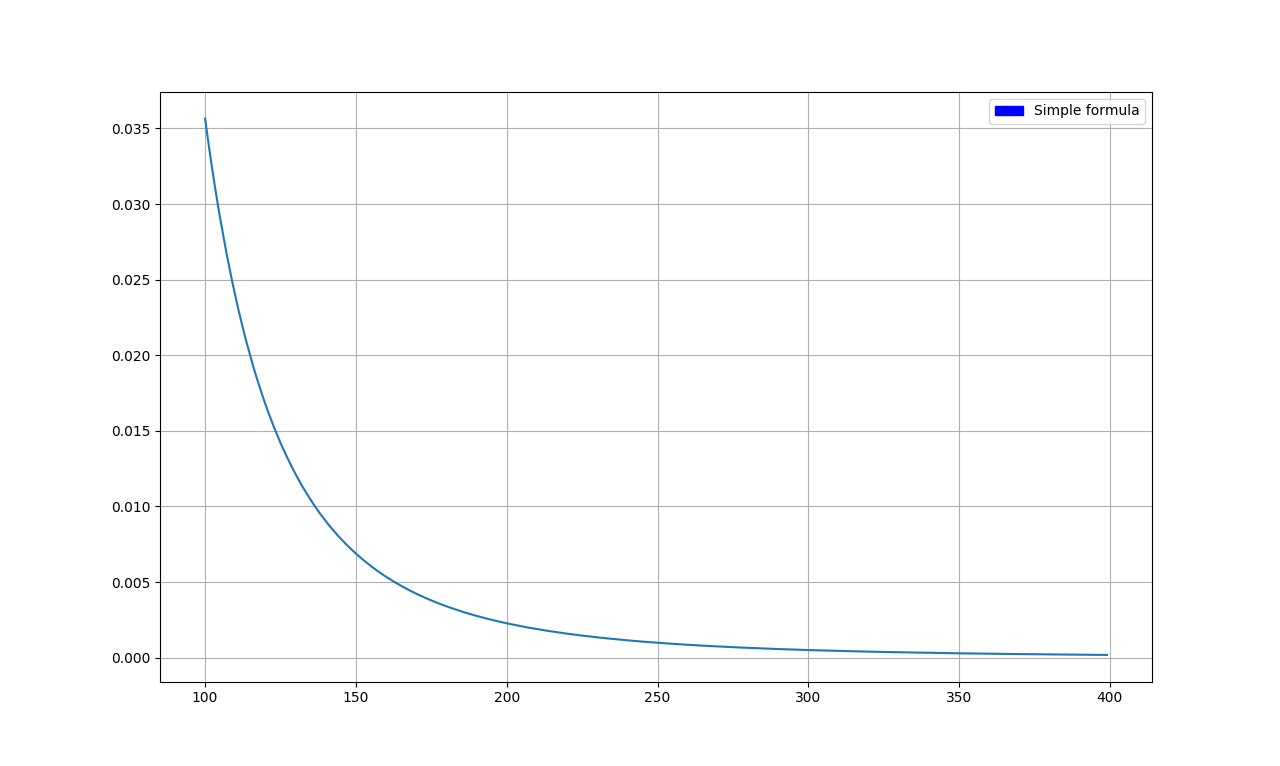
\includegraphics[scale=1.0]{plot.png}

\newpage

Рассмотрим $n$-мерную гиперсферу (гипершар). Исходя из соображений размерности (dimensional analysis) объем гиперсферы должен быть пропорционален $n$-ой степени $R$:
\begin{gather}
	V_n (R) = \int \dots \int_{x_1^2 + \dots x_n^2 \leq R^2} dx_1 \dots dx_n = C_n R^n \notag
\end{gather}

Объем сферы $V_n(R)$ может быть получен путем интегрирования площади сферических слоев $S_{n-1}(R)$ по радиусу сферы:
\begin{gather}
	V_n(R) = \int_{0}^{R} S_{n-1}(r) dr \notag \\
	S_{n-1}(R) = \frac{d V_n(R)}{dR} = nC_n R^{n-1} \notag 
\end{gather}

Таким образом, очевидно, что интеграл по гиперсферическим координатам дает $nC_n$:
\begin{gather}
	\int \dots \int_{x_1^2 + \dots x_n^2 \leq R^2} dx_1 \dots dx_n = n C_n \int_{0}^{R} r^{n-1} dr = \int \dots \int d \Omega_{n-1} \int_{0}^{R} r^{n-1} dr \notag \\
	\int \dots \int d \Omega_{n-1} = n C_n \notag
\end{gather}

Для того, чтобы получить численное выражение для $C_n$ рассмотрим интеграл функции $f(x_1, \dots x_n) = \exp \lb -x_1^2 - \dots x_n^2 \rb$ по всему объему $n$-мерного пространства. Сразу же осуществим переход к гиперсферическим координатам, учитывая вышеизложенные факты:
\begin{gather}
	\int_{-\infty}^{\infty} \dots \int_{-\infty}^{\infty} \exp \lb -x_1^2 - \dots -x_n^2 \rb dx_1 \dots dx_n = \int_{0}^{\infty} \exp \lb -r^2 \rb r^{n-1} dr \int d \Omega_{n-1}  = n C_n \int_{0}^{R} r^{n-1} \exp \lb -r^2 \rb dr= \notag \\
	= \frac{1}{2} \Gamma \lb \frac{n}{2} \rb n C_n \notag
\end{gather}

Одновременно, многомерный интеграл представим в виде произведения одномерных интегралов Пуассона:
\begin{gather}
	\int_{-\infty}^{\infty} \dots \int_{-\infty}^{\infty} \exp \lb -x_1^2 - \dots - x_n^2 \rb d x_1 \dots dx_n = \left[ \int_{-\infty}^{\infty} \exp \lb -x_1^2 \rb dx_1 \right]^n  = \pi^\frac{n}{2} \notag 
\end{gather}

Итак, получаем следующее выражение для $C_n$:
\begin{gather}
	C_n = \frac{\pi^\frac{n}{2}}{\frac{n}{2} \Gamma \lb \frac{n}{2} \rb} \notag
\end{gather}

Рассмотрим интеграл все той же экспоненты, но уже по объему $n$-мерной гиперсферы. Как и раньше, перейдем к гиперсферическим координатам:
\begin{gather}
	\int \dots \int_{x_1^2 + \dots + x_n^2 \leq R^2} \exp \lb -x_1^2 - \dots - x_n^2 \rb dx_1 \dots dx_n = \int_{0}^{R} r^{n-1} \exp \lb -r^2 \rb dr \int d \Omega_{n-1} = \notag \\
	= \frac{2 \pi^{\frac{n}{2}}}{\Gamma \lb \frac{n}{2} \rb} \int_{0}^{R} r^{n-1} \exp \lb -r^2 \rb dr = \left[ t = r^2 \right] = \frac{\pi^{\frac{n}{2}}}{\Gamma \lb \frac{n}{2} \rb} \int_{0}^{R^2} t^{\frac{n}{2} - 1} \exp \lb -t \rb dt = \frac{\pi^{\frac{n}{2}}}{\Gamma \lb \frac{n}{2} \rb} \gamma \lb \frac{n}{2}, R^2 \rb \notag
\end{gather}

\end{document}
